\section{Basis Calculus}\label{cha:tensorEncodings}\label{cha:basisCalculus}

\red{
Basis Calculus stores informations in the selection of basis elements, while coordinate calculus uses the coordinates to each index for storage.
While coordinate calculus is more expressive, basis calculus can be exploited in sparse representations of composed functions.
}

\subsection{Encoding of Subsets and Relations}

Based on the concept of one-hot encodings of states we in this chapter develop the construction of encodings to sets, relations and functions.

\begin{figure}[h]
	\begin{center}
		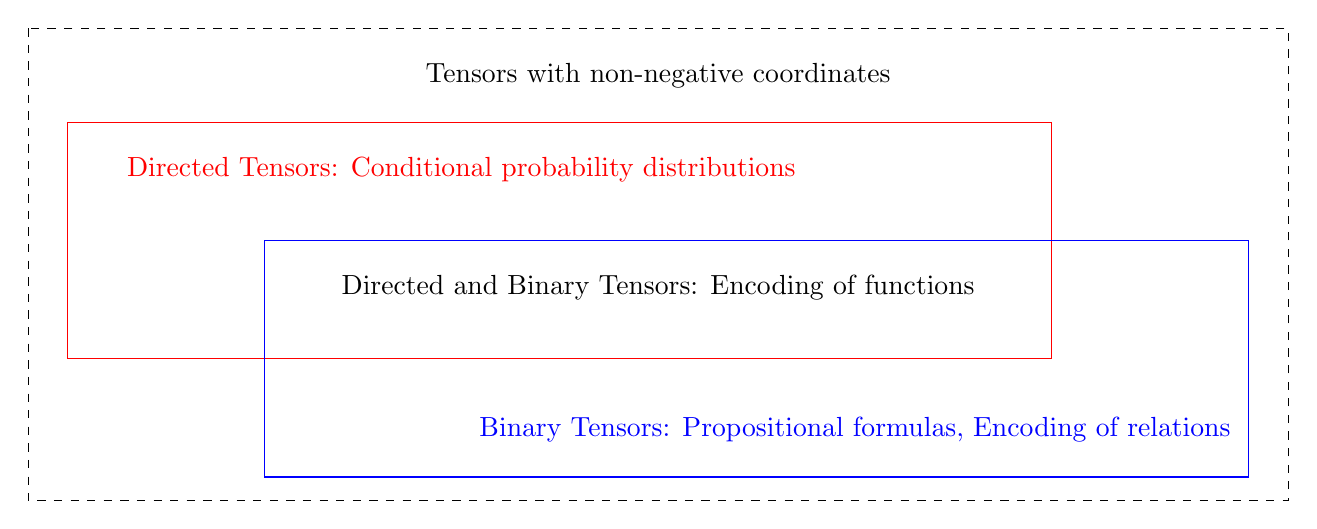
\begin{tikzpicture}[yscale=0.6]
	\draw[dashed] (-10.5,12) rectangle (5.5,2);
	\node[anchor=center] (text) at (-2.5,11) {Tensors with non-negative coordinates};
	
	\draw[red] (-10,10) rectangle (2.5,5); 
	\node[anchor=center,red] (text) at (-5,9) {Directed Tensors: Conditional probability distributions};
	\draw[blue] (-7.5,7.5) rectangle (5,2.5); 
	\node[anchor=center,blue] (text) at (0,3.5) {Binary Tensors: Propositional formulas, Encoding of relations};

	\node[anchor=center] (text) at (-2.5,6.5) {Directed and Binary Tensors: Encoding of functions};
\end{tikzpicture}
	\end{center}
	\caption{Sketch of the tensors with non-negative coordinates. 
	We investigate in this chapter tensors, which are directed and binary.}
\end{figure}


Here we show how we can use binary numbers to encode the truth of set memberships.

\begin{definition}[Subset Encoding]\label{def:subsetEncoding}
	We say that an arbitrary set $\arbset$ is enumerated by a categorical variables $\individualvariableof{\arbset}$ taking values in $[\catdimof{\arbset}]$, when $\catdimof{\arbset}=\absof{\arbset}$ and there is a bijective function
		\[ \indexinterpretationof{} : [\catdimof{\arbset}] \rightarrow \arbset \, . \]
	Given an set $\arbset$ enumerated by the variable $\individualvariableof{\arbset}$, any subset $\arbsubset\subset\arbset$ is encoded by the tensor $\onehotmapto{\arbsubset}[\individualvariable]$ defined for $\catindex\in[\absof{\arbset}]$ as
	%Let there be a set $\arbset$, which elements we enumerate by $x_{\catindex}$ for $\catindex\in[\absof{\arbset}]$, and let there be a categorical variable $\individualvariable$ taking values in $[\absof{\arbset}]$ selecting the members.
	%We define the encoding of a subset $\arbsubset\subset\arbset$ as the tensor $\onehotmapto{\arbsubset}[\individualvariable]$ with coordinates
% \[ \onehotmapto{\arbsubset}[\individualvariable] : \arbset \rightarrow \{0,1\}\]
%	defined for $x\in\arbset$
	\begin{align}
	 	\onehotmapto{\arbsubset}[\individualvariable={\catindex}] = \begin{cases}
		1 & \text{if } \indexinterpretationofat{}{\catindex} \in \arbsubset \\
		0 & \text{else}
		\end{cases} \, . 
	\end{align}
\end{definition}

%	a representation of the set as
%		\[ \arbset = \left\{x_{\catindex} \, : \, \catindex\in[\absof{\arbset}] \right\} \, . \]



% Decomposition
In a one-hot basis decomposition we have
	\[ \onehotmapto{\arbsubset}[\individualvariable] \coloneqq \sum_{\catindex\in[\cardof{\arbset}] \, : \, \indexinterpretationofat{}{\catindex}\in\arbsubset}\onehotmapofat{\catindex}{\individualvariable} \, . \]
%where $\onehotmapof{x}$ denotes the one-hot encoding of an element $x$ with respect to an enumeration of the elements $\arbset$ by $[\catdim]$ or $\facstates$.

% Explanation
Encoding of subsets as vectors: Each coordinate associated with a possible element, $\{0,1\}$ encoding whether in subset.
The encodings is thus a binary tensor.
Any subset encoding is a binary tensor.

\begin{definition}[Relation Encoding]
	Given two finite sets $\inset$, $\outset$, a relation is a subset of their cartesian product
		\[ \exrelation \subset \inset \times \outset \, . \]
	Given an enumeration of $\inset$ and $\outset$ by the categorical variables $\individualvariableof{\insymbol}$ and $\individualvariableof{\outsymbol}$ and interpretation maps 
	$\indexinterpretationof{\insymbol}$, $\indexinterpretationof{\outsymbol}$
	, we define the encoding of this subset as the tensor $\onehotmapto{\exrelation}[\individualvariableof{\insymbol},\individualvariableof{\outsymbol}]$ with the coordinates
	\begin{align}
		\onehotmapto{\exrelation}[\individualvariableof{\insymbol}=\catindexof{\insymbol},\individualvariableof{\outsymbol}=\catindexof{\outsymbol}]
		= \begin{cases}
		1 & \text{if } (\indexinterpretationofat{\insymbol}{\catindexof{\insymbol}},\indexinterpretationofat{\outsymbol}{\catindexof{\outsymbol}}) \in \exrelation \\
		0 & \text{else}
		\end{cases} \, . 
	\end{align}
\end{definition}

% Decomposition
The relation encoding has a decomposition into one-hot encodings as
	\[ \onehotmapto{\exrelation}[\individualvariable_{\insymbol},\individualvariable_{\outsymbol}]
	 = \sum_{\catindexof{\insymbol},\catindexof{\outsymbol} \, : \, (\indexinterpretationofat{\insymbol}{\catindexof{\insymbol}},\indexinterpretationofat{\outsymbol}{\catindexof{\outsymbol}}) \in \exrelation}
	\onehotmapofat{\catindexof{\insymbol}}{\catvariableof{\insymbol}}  \otimes \onehotmapofat{\catindexof{\outsymbol}}{\catvariableof{\outsymbol}}  \, . \]

Relations are subsets of cartesian products and encodings of relations are the encodings of subsets by vectors.
They have a matrix structure by the cartesian product, which can be further folded to tensors, when the sets itself are cartesian products.


\begin{theorem}
	The relational encoding is a bijection between the set of relations and the set of binary tensors.
\end{theorem}
\begin{proof}
	% =>
	By definition, a relational encoding is the encoding of a subset and thus a binary tensor.
	% <= 
	Any matrification of a binary tensor marks by its $1$ coordinates the elements of a relation.
\end{proof}

% Significance
We can thus understand any matrification of a binary tensor as the encoding of a relation and vice versa.



\subsubsection{Higher order relations}


We can extend this contraction to relations of higher order, and arrive at encoding schemes usable for relational databases.

\begin{definition}\label{def:daryRelation}
	Given sets $\arbset^{\atomenumerator}$ for $\atomenumeratorin$, a $\atomorder$-ary relation is a subset of a their cartesian product, that is
		\[ \exrelation \subset  \bigtimes_{\atomenumeratorin} \arbset^{\atomenumerator} \, . \]
	Given an enumeration of each set $\arbset^{\atomenumerator}$ by a variable $\individualvariableof{\atomenumerator}$ and an interpretation map $\indexinterpretationof{\atomenumerator}$, we define the encoding of the relation as the tensor $\onehotmapto{\exrelation}[\individualvariableof{[\atomorder]}]$ with coordinates
	\begin{align}
		\onehotmapto{\exrelation}[\individualvariableof{0}=\catindexof{0},\ldots,\individualvariableof{\atomorder-1}=\catindexof{\atomorder-1}]
		= \begin{cases}
		1 & \text{if } (\indexinterpretationofat{0}{\catindexof{0}},\ldots,\indexinterpretationofat{\atomorder-1}{\catindexof{\atomorder-1}}) \in \exrelation \\
		0 & \text{else}
		\end{cases} \, . 
	\end{align}
\end{definition}


\begin{example}[Propositional Formulas]
	Propositional formulas are equal to the subset encoding of their models.
	The sets $\arbset^{\atomenumerator}$ are all $[2]$ and are interpreted as the possible assignments to the boolean atoms.
\end{example}


\begin{example}[Relational Databases]
	Relational Databases can be encoded as tensors using the relation encoding scheme.
	Each column is thereby understood as a categorical variable, which values form the sets $\arbsetof{\catenumerator}$.
\end{example}

% Sparse Representations
Let us notice, that the dimensionality of the tensor space used for representing a relation is 
	\[ \prod_{\catenumeratorin} \cardof{\arbsetof{\catenumerator}} \]
and therefore growing exponentially with the number of variables.
Relations are however often sparse, in the sense that 
	\[ \cardof{\exrelation} << \prod_{\catenumeratorin} \cardof{\arbsetof{\catenumerator}} \, . \]
It is therefore often benefitially to choose sparse encoding schemes, for example by restricted CP formats (see Chapter~\ref{cha:sparseTC}) to represent $\onehotmapof{\exrelation}$.

\subsection{Encoding of Functions}

Real valued functions are directly tensors by definition.

\subsubsection{Relational Encoding of Functions}

% Reference to first definition
In Definition~\ref{def:functionRepresentation} we have introduced the relational encoding of functions between the states of factored systems.
We now generalize the representation scheme towards maps between arbitrary unstructured sets.

\begin{definition}[Relational Encoding of Maps]\label{def:functionRelationEncoding}
	Any map
		\[ \exfunction : \inset \rightarrow \outset \]
	can be represented by a relation
		\[ \exrelationof{\exfunction} \coloneqq \left\{ (x,\exfunction(x) \, : \, x \in \inset )\right\} \subset \inset \times \outset \, . \]
	Given a enumeration of the sets by $\individualvariableof{\insymbol}$ and $\individualvariableof{\outsymbol}$ we define the relational encoding of $\exfunction$ as the tensor
		\[ \rencodingofat{\exfunction}{\individualvariableof{\insymbol},\individualvariableof{\outsymbol}} = \onehotmapto{\exrelationof{\exfunction}}\left[\individualvariableof{\inset},\individualvariableof{\outset}\right]  \, . \]
\end{definition}

\begin{remark}[Reduction to images]
	% Image enumeration
	When $\exfunction$ maps into a set of infinite cardinality, we restrict $\outset$ to the image of $\exfunction$ and enumerate the image by a variable $\catvariableof{\exfunction}$.
	This scheme is applied, when $\exfunction$ is itself a tensor, i.e. $\outset=\rr$.
	While the variable $\catvariableof{\exfunction}$ can in general be of the same cardinality as the domain set $\inset$, it will be in $[2]$ when considering binary tensors.
\end{remark}

% Characterization of the directed and binary tensors
We notice, that any relational representation of a function is also a directed tensor with incoming variables to the domain and outgoing variables to the image.
It furthermore holds, that the set of directed and binary tensors is characterized by the relational encoding of functions.
This is shown in the next theorem, by the claim that any binary tensor which is directed is the relational representation of a function.

\begin{theorem}\label{the:rencodingDirected}
	Let $\inset,\outset$ be sets and $\exrelation\subset\inset\times\outset$ a relation.
	If and only if there exists a map $\exfunction:\inset\rightarrow\outset$ such that $\exrelation=\exrelationof{\exfunction}$, the relational encoding $\rencodingof{\exfunction}$ is a directed tensor with $\individualvariableof{\insymbol}$ incoming and $\individualvariableof{\outsymbol}$ outgoing.
%	If and only if the relation is a function between domain and image set, its encoding is directed with domain incoming and image outgoing.
\end{theorem}
\begin{proof}
	% =>
	When $\exfunction$ is a function, we have for any $\indindexofin{\insymbol}$
		\[ \sum_{\indindexofin{\outsymbol}} \rencodingofat{\exfunction}{\indexedindvariableof{\insymbol},\indexedindvariableof{\outsymbol}}
		=  \rencodingof{\exfunction}[\indexedindvariableof{\insymbol},\indvariableof{\outsymbol}=\exfunction(\indindexof{\insymbol})] = 1 \, . \]
	% <=
	Conversely let there be a relation $\exrelation$, such that $\rencodingof{\exrelation}$ is directed. %, we construct a map $\exfunction$ with $\exrelation=\exrelationof{\exfunction}$.
	To this end, we observe that for any $\indindexofin{\insymbol}$ the tensor
		\[  \onehotmapofat{\exrelation}{\indexedindvariableof{\insymbol},\indvariableof{\outsymbol}} \]
	is a binary tensor with coordinate sum one and therefore a basis vector.
	It follows that the function $\exfunction : \inset \rightarrow \outset $ 
		\[ \exfunction(\indindexof{\insymbol}) = \invonehotmapof{\onehotmapofat{\exrelation}{\indexedindvariableof{\insymbol},\indvariableof{\outsymbol}} } \]
	is well-defined.
	We then have by construction
	\begin{align*}
		\rencodingof{\exfunction} 
		= \sum_{\indindexofin{\insymbol}} \onehotmapof{\indindexof{\insymbol}} \otimes \onehotmapof{\exfunction(\indindexof{\insymbol})}
		=  \sum_{\indindexofin{\insymbol}} \onehotmapof{\indindexof{\insymbol}} \otimes \onehotmapofat{\exrelation}{\indexedindvariableof{\insymbol},\indvariableof{\outsymbol}} 
		= \onehotmapof{\exrelation}
	\end{align*}
	and therefore $\exrelation = \exrelationof{\exfunction}$.
%	 with a directed encoding, directionality implies that for any $\incatindex$ there is exactly one $\outcatindex$ such that $\onehotmapto{\exrelation}[\indexedcatvariableof{\insymbol}\indexedcatvariableof{\outsymbol}]=1	
%	Then we define a function $\exfunction$ as the mapping of $\incatindex$ to the corresponding $\outcatindex$ with $\onehotmapto{\exrelation}[\incatindex\outcatindex]=1$ and observe $\exrelation=\exrelationof{\exfunction}$.
\end{proof}

% Grid sets
We are specially interested in sets of states of a factored system, which amounts to the case in Definition~\ref{def:functionRepresentation}.
Those state sets have a decomposition into a cartesian product of $\atomorder$ sets
	\[ \arbset = \facstates \, . \]
The most obvious enumeration of the set $\arbset$ is therefore by the collection of state variables $\{\catvariableof{\atomenumerator} \, : \, \atomenumeratorin \}$.
Functions between states of factored systems with $\atomorder_{\insymbol}$ and $\atomorder_{\outsymbol}$ state variables can be represented by $\atomorder_{\insymbol}+\atomorder_{\outsymbol}$-ary relations and Definition~\ref{def:functionRelationEncoding} has an obvious generalization to this case with multiple enumeration variables.


% Conditional 
Since the relational encoding of any map between factored systems is directed, it can be interpreted by a conditional probability tensor, as we state next.

%% Maps
\begin{corollary}%\label{the:condProbFunctionRepresentation}
	The relational encoding $\rencodingof{\exfunction}$ (see Definition~\ref{def:functionRepresentation}) of a function $\exfunction$ between factored systems is a conditional probability tensor, where the legs to the image system are the conditions and the legs to the target system the distribution legs.
\end{corollary}
%\begin{proof}
%	To proof the claim we need to show that contracting the trivial tensor to the target legs results in the trivial tensor of the image legs, that is
%		\[ \onesof{\shortcatvariables} = \contractionof{\{\rencodingof{\exfunction}\}}{\shortcatvariables} \, . \]
%	This can be shown coordinatewise by sums over the target legs as
%	\begin{align*}
%		\sum_{\seccatindices} \ftensorof{\exfunction}_{\seccatindices,:}
%		 	= &  \sum_{\seccatindices} \sum_{\catindices}  \left(\onehotmapof{\exfunction(\catindices)}\right)_{\seccatindices} \otimes \onehotmapof{\catindices} \\
%			= &  \sum_{\catindices} \onehotmapof{\catindices}  \\
%			= &  \onesof{\shortcatvariables}  \, .
%	\end{align*}
%	Here we used in the second equality, that the function $\exfunction$ maps each index pair $(\catindices)$ of the image system to exactly one index pair $(\seccatindices)$ in the target system.
%	In the third equality we further used that the sum of the one-hot encodings of all states is the trivial tensor.
%\end{proof}

%% Deterministic by construction
These are deterministic conditional probability tensors, in the sense that any slice with respect to the input variables is a basis tensor.
Through contractions with distribution tensors (e.g. distributions in domain systems) they get stochastic.
This is for example the case in the empirical distribution, which can be understood as the forwarding of the uniform distribution on the sample enumeration.








\subsection{Calculus of relational encodings}



\subsubsection{Function Evaluation}

\begin{theorem}[Basis Calculus]\label{the:basisCalculus}
	Retrieving the value of the function at a specific state is then the contraction of the tensor representation with the one-hot encoded state.
	For any state indexed by $(\catindices)$ we have
		\[ \onehotmapofat{\exformula(\catindices)}{\catvariableof{\exformula}} 
		= \contractionof{\{\rencodingof{\exformula},\onehotmapof{\catindices}\}}{\catvariableof{\exformula}} \, .\]
	Thus, we can retrieve the function evaluation by the inverse one-hot mapping as
		\[ \exformula(\catindices) 
		= \invonehotmapof{\contractionof{\{\rencodingof{\exformula},\onehotmapof{\catindices}\}}{\catvariableof{\exformula}}} \, . \]
	This generalizes Example~\ref{exa:atomicFunction} to arbitrary maps between factored systems.
\end{theorem}
\begin{proof}
	By doing the summation in tensor product notation.
\end{proof}

%% Usage: Basis Calculus
We can thus use tensor contractions to calculate the values of functions.
Since basis vectors being the one-hot encoding of the domain system are mapped to basis vectors being the encoding of the image system, we call these contraction basis calculus.

\subsubsection{Composition of function}

We have already used, that combination of propositional formulas by connectives can be represented by contractions.
In a more general perspective, any composition of functions between factored systems is in its relational encoding the contraction of the encoded functions.

\begin{theorem}[Composition of Functions]\label{the:compositionByContraction}
	Let there be two maps between factored systems 
		\[ \exfunction : \bigtimes_{\node\in\nodes_1} [\catdimof{\node}] \rightarrow \bigtimes_{\node\in\nodes_2} [\catdimof{\node}] \]
	and 
		\[ \secexfunction : \bigtimes_{\node\in\nodes_2} [\catdimof{\node}] \rightarrow \bigtimes_{\node\in\nodes_3} [\catdimof{\node}] \]
	with the image system of $\exfunction$ is the domain system of $\secexfunction$.
	Then the relational encoding of the composition 
		\[ \secexfunction(\exfunction) :  \bigtimes_{\node\in\nodes_1} [\catdimof{\node}] \rightarrow \bigtimes_{\node\in\nodes_3} [\catdimof{\node}] \]
	satisfies
		\[ \rencodingof{\secexfunction(\exfunction)} = \contractionof{\{\rencodingof{\exfunction},\rencodingof{\secexfunction}\}}{\nodes_1\cup\nodes_3} \, .  \]
\end{theorem}
\begin{proof}
	By definition we have
	\begin{align*}
		\rencodingof{\secexfunction(\exfunction)} = \sum_{i_1 \in \bigtimes_{\node\in\nodes_1} [\catdimof{\node}]} \onehotmapof{i_1} \otimes \onehotmapof{\secexfunction(\exfunction(i_1))} \, ,
	\end{align*}
	where by $i_1$ we denote in a slide abuse of notation the tuple indexing the state of the domain factored systems of $\exfunction$.
	On the other side, we have that
	\begin{align*}
	 	\contractionof{\{\rencodingof{\exfunction},\rencodingof{\secexfunction}\}}{\catvariableof{\nodes_1}\catvariableof{\nodes_3}} 
		& =
		\sum_{\tilde{i}_2 \in \bigtimes_{\node\in\nodes_2}[\catdimof{\node}]} 
		\left( \sum_{i_1 \in \bigtimes_{\node\in\nodes_1}[\catdimof{\node}]}  \onehotmapof{i_1} \cdot \left(\onehotmapof{\exfunction(i_1)}\right)_{\tilde{i}_2} \right)
		\left( \sum_{i_2 \in \bigtimes_{\node\in\nodes_2}[\catdimof{\node}]}  \left(\onehotmapof{i_2}\right)_{\tilde{i}_2} \cdot \onehotmapof{\secexfunction(i_2)} \right) \\
		& = 
		\sum_{\tilde{i}_2 \in \bigtimes_{\node\in\nodes_2}[\catdimof{\node}]} 
		\left( \sum_{i_1 \in \bigtimes_{\node\in\nodes_1}[\catdimof{\node}]}  \onehotmapof{i_1} \cdot \delta_{\exfunction(i_1),\tilde{i}_2} \right)
		\left( \sum_{i_2 \in \bigtimes_{\node\in\nodes_2}[\catdimof{\node}]}  \delta_{i_2 \tilde{i}_2} \cdot \onehotmapof{\secexfunction(i_2)} \right) \\
		& = 
		\sum_{i_1 \in \bigtimes_{\node\in\nodes_1}[\catdimof{\node}]}
		\sum_{\tilde{i}_2 \in \bigtimes_{\node\in\nodes_2}[\catdimof{\node}]}  \delta_{\exfunction(i_1),\tilde{i}_2} \cdot \left(  \onehotmapof{i_1}   \otimes \onehotmapof{\secexfunction(i_2)} \right) \\
		& = 
		\sum_{i_1 \in \bigtimes_{\node\in\nodes_1} [\catdimof{\node}]} 
		\onehotmapof{i_1} \otimes \onehotmapof{\secexfunction(\exfunction(i_1))} \, .
	\end{align*}
	Here we represented the contraction of the variables in $\nodes_2$ by the summation over another index $i_2$.
	In the last equation we used that the delta tensor does not vanish only for $\tilde{i}_2= \exfunction(i_1)$.
	The claim follows, since both expressions are equal.
\end{proof}

% Iterative usage
We can use Theorem~\ref{the:compositionByContraction} iteratively to further decompose the function $\secexfunction$.
In this way, the relational encoding of a function consistent of multiple compositions can be represented as the contractions of all the functions.
The relational encoding of propositional formulas for instance can in this way be represented as a contraction of the encodings of its logical connectives applied on the respective formula spaces. 
%It is thereby of central importance that for any connective a respective variable is added, which then disappears in the contractions.




\subsubsection{Compositions with real functions}

\red{Follows from composition calculus above with the usage of }
	\[ \hypercore = \sbcontractionof{\rencodingof{\hypercore}, \restrictionofto{Id}{\imageof{\hypercore}} }{\shortcatvariables} \, . \]

We here investigate how the composition of a tensor 
	\[ \hypercore : \facstates \rightarrow \rr \]
with arbitrary functions 
	\[ \chainingfunction: \rr \rightarrow \rr \]
can be represented.
This is for example relevant, when representing the distributions of an exponential family.

% Strategy
Our main strategy is in understanding the tensor $\hypercore$ as a map to its finite image, seen as the enumerated states of a categorical variable building a factored system.
We then use the relational encoding $\rencodingof{\hypercore}$ of this map between factored systems. 

By $\restrictionofto{\chainingfunction}{\mathcal{M}}$ we further denote the restriction of a real function $\chainingfunction$ to an enumerated set $\mathcal{M} =\{x_i \, : \, i \in [\cardof{\mathcal{M}}]\} \subset \rr$, i.e. the vector
	\[ \restrictionofto{\chainingfunction}{\mathcal{M}} : [\cardof{\mathcal{M}}] \rightarrow \rr \]
defined for $i \in [\cardof{\mathcal{M}}]$ as
	\[ \restrictionofto{\chainingfunction}{\mathcal{M}}(i) = \chainingfunction(x_i) \, . \]


\begin{theorem}\label{the:tensorFunctionComposition}
	We have for any tensor $\hypercore$ and real function $\chainingfunction$ (see Figure~\ref{fig:tensorFunctionComposition})
		\[ \chainingfunction\circ\hypercore = \contractionof{\{\rencodingof{\hypercore}, \restrictionofto{\chainingfunction}{\imageof{\hypercore}}\}}{\shortcatvariables} \, . \]
\end{theorem}
\begin{proof}
	We enumerate the image $\mathrm{im}(\hypercore)$ by $\{x_i \, : \, i \in [\cardof{\mathrm{im}(\hypercore)}]\}$.
	For arbitrary but fixed $\catindices\in\facstates$ let $\tilde{i}$ be such that $\hypercore(\catindices) = x_i$.
	Then we have for $\randomxof{\hypercore}$ denoting the image variable of $\rencodingof{\hypercore}$ that
		\[ \contractionof{\{\rencodingof{\hypercore},\onehotmapof{\catindices}\}}{\{\randomxof{\hypercore}\}} = \onehotmapof{\tilde{i}} \]
	and
		\[ \contractionof{\{\rencodingof{\hypercore}, \restrictionofto{\chainingfunction}{\imageof{\hypercore}}, \onehotmapof{\catindices}\}}{\varnothing} = 
		\contractionof{\{\restrictionofto{\chainingfunction}{\imageof{\hypercore}}, \onehotmapof{\tilde{i}}\}}{\varnothing} = 
		\chainingfunction(\hypercore(\catindices)) \, . 
		\]
	Since $\catindices$ was chosen arbitrarly form $\facstates$, this shows that $\chainingfunction\circ\hypercore$ and $ \contractionof{\{\rencodingof{\hypercore}, \restrictionofto{\chainingfunction}{\imageof{\hypercore}}\}}{\shortcatvariables}$ coincide on all inputs and are thus equal.
\end{proof}

\begin{figure}[h]
\begin{center}
	\begin{tikzpicture}[scale=0.35] % , baseline = -3.5pt




\begin{scope}[shift={(-15,0)}]

\drawatomcore{-6}{-8}{$\chainingfunction\circ\hypercore$}


	\begin{scope}[shift={(-6,-12)}]
		\draw[] (0,1)--(0,-1) node[midway,left] {\tiny $\catvariableof{0}$}; 
		\draw[] (1.5,1)--(1.5,-1) node[midway,left] {\tiny $\catvariableof{1}$}; 
		\node[anchor=center] (text) at (3,0) {$\cdots$};
		\draw[] (4,1)--(4,-1) node[midway,right] {\tiny $\catvariableof{\atomorder\shortminus1}$}; 
	\end{scope}

\end{scope}



%\node[anchor=center] (text) at (-14.25,-10) {${=}$};



%\begin{scope}[shift={(-12.5,0)}]
%
%\node[anchor=center] (text) at (1,-7.25) {\small $\chainingfunction$};
%\draw (5.5,-7.25) ellipse (6 and 4.5);
%
%
%\drawatomcore{3.5}{-8}{$\ftensorof{\exformula}$}
%\drawatomindices{3.5}{-12}	
%\draw[] (5.5,-9)--(5.5,-7) node[midway,right] {\tiny $\randomxof{\hypercore}$};
%
%
%\draw (4.75,-3.5) rectangle (6.25,-7);
%\node[anchor=center] (text) at (5.5,-5.25) {$\begin{bmatrix} 
%0 \\
%1
%\end{bmatrix}$};
%
%\end{scope}


\begin{scope}[shift={(-12.5,0)}]

\node[anchor=center] (text) at (-0.5,-10) {${=}$};

%\node[anchor=center] (text) at (0.5,-8) {$\mathrm{log}$};

\drawatomcore{3.5}{-8}{$\rencodingof{\hypercore}$}
\drawatomindices{3.5}{-12}	
\draw (5.5,-9)--(5.5,-6) node[midway,right] {\tiny $\randomxof{\hypercore}$};
\draw[->] (5.5,-9) -- (5.5,-7.5);

\draw (3.25,-4) rectangle (7.5,-6);
\node[anchor=center] (text) at (5.5,-5) {$\restrictionofto{\chainingfunction}{\imageof{\hypercore}}$
%\begin{bmatrix} 
%	\chainingfunction(0) \\
%	\chainingfunction(1)
%\end{bmatrix}
};

\end{scope}

\end{tikzpicture}
\end{center}
\caption{Representation of the composition of a tensor $\hypercore$ with a real function $\chainingfunction$.}
\label{fig:tensorFunctionComposition} 
\end{figure}


\begin{corollary}\label{cor:rhoToNormal}
	For any tensor $\hypercoreat{\shortcatvariables}$ we have
		\[ \hypercoreat{\shortcatvariables} = \contractionof{\rencodingof{\hypercore},\idrestrictedto{\imageof{\hypercore}}}{\shortcatvariables} \, . \]
\end{corollary}
\begin{proof}
	Directly by using $\chainingfunction=\mathrm{Id}$.
\end{proof}


\begin{corollary}\label{cor:onesHead}
	For any tensor $\hypercore$, which is directed with $\shortcatvariables$ incoming, we have
		\[ \onesat{\shortcatvariables} = \contractionof{\rencodingof{\hypercore}}{\shortcatvariables} \, . \]
\end{corollary}
\begin{proof}
	Directly by using $\chainingfunction=\ones$.
\end{proof}

% Replacement of Slicing Theorem
\begin{corollary}\label{cor:directedTrafo}
	Let $\basisslices$ be a directed and binary tensor with incoming variables being $\shortcatvariables$, and $\gentensor$ a tensor, which variables are the outgoing variables of $\basisslices$.
	Let further $\coordinatetrafo:\rr\rightarrow\rr$ be any real function.
	Then
		\[ \coordinatetrafo \circ \contractionof{\{\basisslices,\gentensor\}}{\shortcatvariables} 
		= \contractionof{\{\basisslices,\coordinatetrafo\circ \gentensor\}}{\shortcatvariables} \, . \]
\end{corollary}
\begin{proof}
	Since $\basisslices$ is a directed and binary tensor, we find a map
		\[ \exfunction : \facstates \rightarrow \secfacstates \]
	such that $\basisslices=\rencodingof{\exfunction}$ and a map $V$ such that $\gentensor=\restrictionofto{V}{\imageof{\exfunction}}$.
	Then Theorem~\ref{the:tensorFunctionComposition} implies that 
		\[ \contractionof{\{\basisslices,\gentensor\}}{\shortcatvariables} = V \circ \exfunction \, . \]
	It follows that 
	\begin{align*}
		\coordinatetrafo \circ \contractionof{\{\basisslices,\gentensor\}}{\shortcatvariables} = \coordinatetrafo \circ V \circ \exfunction 
	\end{align*}
	and by another application of Theorem~\ref{the:tensorFunctionComposition} that
	\begin{align*}
		\coordinatetrafo \circ V \circ \exfunction
		& = \contractionof{\rencodingof{\exfunction}, \restrictionofto{\coordinatetrafo \circ V}{\imageof{\exfunction}}}{\shortcatvariables} \\
		& = \contractionof{\{\basisslices,\coordinatetrafo\circ\gentensor\}}{\shortcatvariables} \, . 
	\end{align*}
	The claim follows as a combination of both equations.
\end{proof}



\begin{example}[Shannon entropy of empirical distribution]
%\begin{theorem}
	The Shannon entropy of an empirical distribution can be efficiently computed by contraction of the datatensor with itself along the atom indices, then applying a coordinatewise $\ln$ and averaging.
%\end{theorem}

%\begin{proof}
	This follows from commutations of contraction and coordinatewise contraction (see Corollary~\ref{cor:directedTrafo}), using that the datacores are directed. 
	%Theorem~\ref{the:CoordinateTransform}, since the datatensor is a slicewise basis tensor.
	To be more precise, let $\secdatamap$ be a copy of $\datamap$ with identical image space and copied domain space.
	Then $\secdatacoreof{\atomenumerator}$ are tensor cores with identical outgoing legs to $\datacoreof{\atomenumerator}$, but different incoming legs.
	We have that
	\begin{align*}
		\sentropyof{\empdistribution} 
		& = \contractionof{\{\datacoreof{\atomenumerator}\, : \, \atomenumeratorin\} \cup \{\frac{1}{\datanum}\ones \} \cup \{-\ln \contractionof{\{\secdatacoreof{\atomenumerator}\, : \, \atomenumeratorin\} \cup \{\frac{1}{\datanum}\ones \}}{\shortcatvariables} \} }{\varnothing} \\
		& = \contractionof{
		 \left\{\frac{1}{\datanum}\ones, -\ln \contractionof{\{\datacoreof{\atomenumerator},\secdatacoreof{\atomenumerator}\, : \, \atomenumeratorin\} \cup \{\frac{1}{\datanum}\ones \}}{\shortcatvariables} \right\}
		}{\varnothing}
	\end{align*}
	where in the second equation we used Corollary~\ref{cor:directedTrafo}.
%\end{proof}
\end{example}

\subsubsection{Decomposition in case of structured images}

\red{Here the introduction of multiple head variables, i.e. when}
	\[ \outset = \bigtimes_{\catenumeratorin} \arbsetof{\catenumerator}\]
\red{This is the case for the empirical distributions!}


When the image admits a cartesian representation, the relational encoding can be represented by a contraction of relational encodings to each image coordinate.

\begin{theorem}\label{the:functionDecompositionBasisCP}
	Let $\exfunction$ be a function between factored systems
		\[ \exfunction : [\catdim] \rightarrow  \facstates \]
	and denote by
		\[ \exfunction^\atomenumerator : [\catdim] \rightarrow [\catdimof{\atomenumerator}]\]
	the restrictions of $\exfunction$ to axes of $\facstates$.
	We assign the variable $\catvariable$ to the factored system in the domain system of $\exfunction$ and the variables $\catvariableof{\atomenumerator}$ for $\atomenumeratorin$ to the image system of $\exfunction$.
	
	We then have
	\begin{align*}
		\rencodingofat{\exfunction}{\catvariable,\shortcatvariables}  
		= \contractionof{
		\{\rencodingofat{\exfunction^{\atomenumerator}}{\catvariable,\catvariableof{\atomenumerator}} : \atomenumeratorin \} 
		}{\catvariable,\shortcatvariables} \, . 
	\end{align*}
%	and 
%		\[ \baspluscprankof{\rencodingof{\exfunction}} \leq \catdim \, . \]
\end{theorem}
\begin{proof}
	
	We have 
	\begin{align*}
		\rencodingofat{\exfunction}{\catvariable,\shortcatvariables}  
		= \contractionof{
		\{\rencodingofat{\exfunction^{\atomenumerator}}{\catvariable,\catvariableof{\atomenumerator}} : \atomenumeratorin \} 
		}{\catvariable,\shortcatvariables}
	\end{align*}
	since for any $\catindex\in[\catdim]$ 
	\begin{align*}
		\rencodingofat{\exfunction}{\catvariable=\catindex,\shortcatvariables}  
		= \bigotimes_{\atomenumeratorin} \rencodingofat{\exfunction^{\atomenumerator}}{\catvariable=\catindex,\catvariableof{\atomenumerator}}
		= \contractionof{
		\{\rencodingofat{\exfunction^{\atomenumerator}}{\catvariable,\catvariableof{\atomenumerator}} : \atomenumeratorin \} 
		}{\catvariable=\catindex,\shortcatvariables} \, . 
	\end{align*}
	
	To get a representation in the basis CP format, we rename the variable $\catvariable$ in the cores $\rencodingofat{\exfunction^{\atomenumerator}}{\catvariable,\catvariableof{\atomenumerator}}$ by $\decvariable$ and observe that for a trivial scalar core $\onesat{\decvariable}$ 
	\begin{align*}
		\contractionof{
		\{\rencodingofat{\exfunction^{\atomenumerator}}{\catvariable,\catvariableof{\atomenumerator}} : \atomenumeratorin \} 
		}{\catvariable,\shortcatvariables} 
		=
		\contractionof{ 
		\{\onesat{\decvariable}\} \cup \{\rencodingofat{\exfunction^{\atomenumerator}}{\decvariable,\catvariableof{\atomenumerator}} : \atomenumeratorin \} \cup \{\identityat{\catvariable,\decvariable}\}
		}{\catvariable,\shortcatvariables}  \, . 
	\end{align*}
	
%	It suffices to show for any $\catindex\in[\catdim]$ we have
%		\[ \contractionof{\{\ftensorof{\exfunction},\onehotmapof{\catindex}\}}{\shortcatvariables} = 
%		 	\contractionof{\{\ftensorof{\exfunction^\atomenumerator} \, : \, \atomenumeratorin\}\cup\{\onehotmapof{\catindex}\}}{\shortcatvariables} \, . 
%		  \]
%	But this holds, since
%	\begin{align*} 
%		\contractionof{\{\ftensorof{\exfunction},\onehotmapof{\catindex}\}}{\shortcatvariables} 
%			& = \bigotimes_{\atomenumeratorin} \onehotmapof{\exfunction^{\atomenumerator}(\catindex)} \\
%			& = \bigotimes_{\atomenumeratorin} \contractionof{\{\ftensorof{\exfunction^\atomenumerator},\onehotmapof{\catindex}\}}{\randomxof{\atomenumerator}} \\
%			& = \contractionof{\{\ftensorof{\exfunction^\atomenumerator} \, : \, \atomenumeratorin \}\cup\{\onehotmapof{\catindex}\}}{\shortcatvariables} \, .
%	\end{align*}
\end{proof}





\subsection{Effective Calculus}\label{sec:effectiveCalculus} % -> Part III

% Calculus against the direction
For specific functions, slices of the relational encodings with respect to head variables are basis vectors.
In that case, we can perform basis calculus in the inverse direction than suggested by the directions of the tensors.
We examplify this situation in the following theorem for relational encodings of logical conjunctions and negations.

\begin{figure}
\begin{center}
	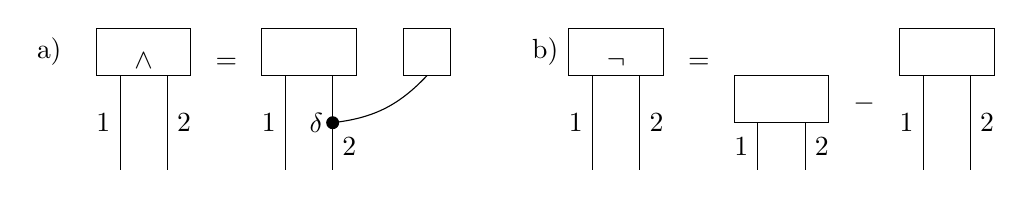
\begin{tikzpicture}[scale=0.3] 

\node at (-12,2) [above]  {a)};

	\begin{scope}[shift={(-7,0)}]
	  	\draw[]  (-3,2) rectangle (1,4);
		\node at (-1,1.9) [above] {${\exformula\land\secexformula}$};
		\draw (-2,2) -- (-2,-2) node[midway,left] {$\catvariableof{1}$};
		\draw (0,2) -- (0,-2) node[midway,right] {$\catvariableof{2}$};	
	\end{scope}
	\node at (-4.5,1.9) [above] {$=$};	
  	\draw[] (-3,2) rectangle (1,4);
	\node at (-1,1.9) [above] {${\exformula}$};
  	\draw[] (3,2) rectangle (5,4);
	\node at (4,1.9) [above] {${\secexformula}$};
	
	\node at (0,0) [left,] {$\delta$};
	\draw[]  (0,2) -- (0,0);% node[midway,left] {$\placeholderof{1}$};
	\draw[fill,] (0,0) circle (0.25cm);
	\draw[] (0,0) -- (0,-2) node[midway,right] {$\catvariableof{2}$};
	\draw[] (4,2) to[bend left=20] (0,0);
	\draw[] (-2,2) -- (-2,-2) node[midway,left] {$\catvariableof{1}$};

\begin{scope}[shift={(27,0)}]
	\node at (-18,2) [above]  {b)};
  	\begin{scope}[shift={(-14,0)}]
	  	\draw[]  (-3,2) rectangle (1,4);
		\node at (-1,1.9) [above] {${\lnot\exformula}$};
		\draw (-2,2) -- (-2,-2) node[midway,left] {$\catvariableof{1}$};
		\draw (0,2) -- (0,-2) node[midway,right] {$\catvariableof{2}$};	
	\end{scope}
	
    	\begin{scope}[shift={(-2,-2)}]
  		\draw[] (-8,2) rectangle (-4,4);
		\node at (-6,2) [above,] {$\ones$};
		\draw[] (-7,2) -- (-7,0) node[midway,left] {$\catvariableof{1}$};
		\draw[] (-5,2) -- (-5,0) node[midway,right] {$\catvariableof{2}$};
	\end{scope}
	
	\draw[] (-2,2) -- (-2,-2) node[midway,left] {$\catvariableof{1}$};
	\draw[](0,2) -- (0,-2) node[midway,right] {$\catvariableof{2}$};
	\node[] at (-4.5,0) [above] {$-$};



	\node at (-11.5,1.9) [above] {$=$};	
	
  	\draw[]  (-3,2) rectangle (1,4);
	\node at (-1,1.9) [above] {${\exformula}$};	
	
\end{scope}

\end{tikzpicture}
\end{center}
\caption{Decomposition schemes by effecitve calculus. a) Conjunction, b) Negations.}\label{fig:ConNegDecomposition}
\end{figure}

\begin{theorem}\label{the:effectiveConjunction}
	For any formulas $\exformula,\secexformula$ we have
	\begin{align*}
		\sbcontractionof{
			\rencodingofat{\land}{\catvariableof{\exformula\land\secexformula},\catvariableof{\exformula},\catvariableof{\secexformula}},\onehotmapofat{1}{\catvariableof{\exformula\land\secexformula}}
		}{\catvariableof{\exformula},\catvariableof{\secexformula}}
		= \onehotmapofat{1}{\catvariableof{\exformula}} \otimes \onehotmapofat{1}{\catvariableof{\secexformula}} \, . 
	\end{align*}
	In particular, it holds that (see Figure~\ref{fig:ConNegDecomposition}a)
	\begin{align*}
		(\exformula\land\secexformula)[\shortcatvariables] = \sbcontractionof{\exformula,\secexformula}{\shortcatvariables} \, . 
	\end{align*}
\end{theorem}
\begin{proof}
	We decompose 
	\begin{align*}
		\rencodingofat{\land}{\catvariableof{\exformula\land\secexformula},\catvariableof{\exformula},\catvariableof{\secexformula}}
		= \onehotmapofat{1}{\catvariableof{\exformula\land\secexformula}} \otimes \onehotmapofat{1}{\catvariableof{\exformula}} \otimes \onehotmapofat{1}{\catvariableof{\secexformula}}
		+ \onehotmapofat{0}{\catvariableof{\exformula\land\secexformula}} \left( \onesat{\catvariableof{\exformula},\onesat{\catvariableof{\secexformula}}} -  \onehotmapofat{1}{\catvariableof{\exformula}} \otimes \onehotmapofat{1}{\catvariableof{\secexformula}} \right) 
	\end{align*}
	and get the first claim as
	\begin{align*}
		\sbcontractionof{
			\rencodingofat{\land}{\catvariableof{\exformula\land\secexformula},\catvariableof{\exformula},\catvariableof{\secexformula}},\onehotmapofat{1}{\catvariableof{\exformula\land\secexformula}}
		}{\catvariableof{\exformula},\catvariableof{\secexformula}}
		& = \sbcontractionof{
			\onehotmapofat{1}{\catvariableof{\exformula\land\secexformula}} \otimes \onehotmapofat{1}{\catvariableof{\exformula}} \otimes \onehotmapofat{1}{\catvariableof{\secexformula}},\onehotmapofat{1}{\catvariableof{\exformula\land\secexformula}}
		}{\catvariableof{\exformula},\catvariableof{\secexformula}} \\
		& = \onehotmapofat{1}{\catvariableof{\exformula}} \otimes \onehotmapofat{1}{\catvariableof{\secexformula}} \, . 
	\end{align*}
	To show the second claim we use
	\begin{align*}
		(\exformula\land\secexformula)[\shortcatvariables] 
		&= \sbcontractionof{
			\rencodingofat{\exformula}{\catvariableof{\exformula},\shortcatvariables},
			\rencodingofat{\secexformula}{\catvariableof{\secexformula},\shortcatvariables},
			\rencodingofat{\land}{\catvariableof{\exformula\land\secexformula},\catvariableof{\exformula},\catvariableof{\secexformula}},
			\onehotmapofat{1}{\catvariableof{\exformula\land\secexformula}}
			}{\shortcatvariables} \\
		&  = \sbcontractionof{
			\rencodingofat{\exformula}{\catvariableof{\exformula},\shortcatvariables},
			\rencodingofat{\secexformula}{\catvariableof{\secexformula},\shortcatvariables},
			(\onehotmapofat{1}{\catvariableof{\exformula}}\otimes \onehotmapofat{1}{\catvariableof{\secexformula}})
			%\rencodingofat{\land}{\catvariableof{\exformula},\catvariableof{\secexformula},\catvariableof{\exformula\land\secexformula}}
			}{\shortcatvariables} \\
		&= \sbcontractionof{\exformula,\secexformula}{\shortcatvariables} \, . 
	\end{align*}
\end{proof}

A similar decomposition holds for negations, as we show next.

\begin{theorem}
	For any formula $\exformula$ we have
	\begin{align*}
		\sbcontractionof{
			\rencodingofat{\lnot}{\catvariableof{\exformula},\catvariableof{\lnot\exformula}},\onehotmapofat{1}{\catvariableof{\lnot\exformula}}
		}{\catvariableof{\exformula}}
		= \onehotmapofat{0}{\catvariableof{\exformula}} =  \onesat{\catvariableof{\exformula}} - \onehotmapofat{1}{\catvariableof{\exformula}} \, . 
	\end{align*}
	and
	\begin{align*}
		\sbcontractionof{
			\rencodingofat{\lnot}{\catvariableof{\exformula},\catvariableof{\lnot\exformula}},\onehotmapofat{0}{\catvariableof{\lnot\exformula}}
		}{\catvariableof{\exformula}}
		= \onehotmapofat{1}{\catvariableof{\exformula}} \, . 
	\end{align*}
	In particular, it holds that (see Figure~\ref{fig:ConNegDecomposition}b)
	\begin{align*}
		(\lnot\exformula)[\shortcatvariables] = \onesat{\shortcatvariables} - \formulaat{\shortcatvariables}  \, . 
	\end{align*}
\end{theorem}
\begin{proof}
	Using that for two dimensional variables we have $\onesat{\catvariable}=\onehotmapofat{0}{\catvariable}+\onehotmapofat{1}{\catvariable}\, .$
\end{proof}

% Usage
These theorems provide a mean to represent logical formulas by sums of one-hot encodings.
Since any propositional formula can be represented by compositions of negations and conjunctions, they are universal.
We further notice, that the resulting decomposition is a basis+ CP format, as further discussed in Chapter~\ref{cha:sparseTC}.
In Figure~\ref{fig:DecompositionExample} we provide an example of this decomposition.


\begin{figure}
\begin{center}
	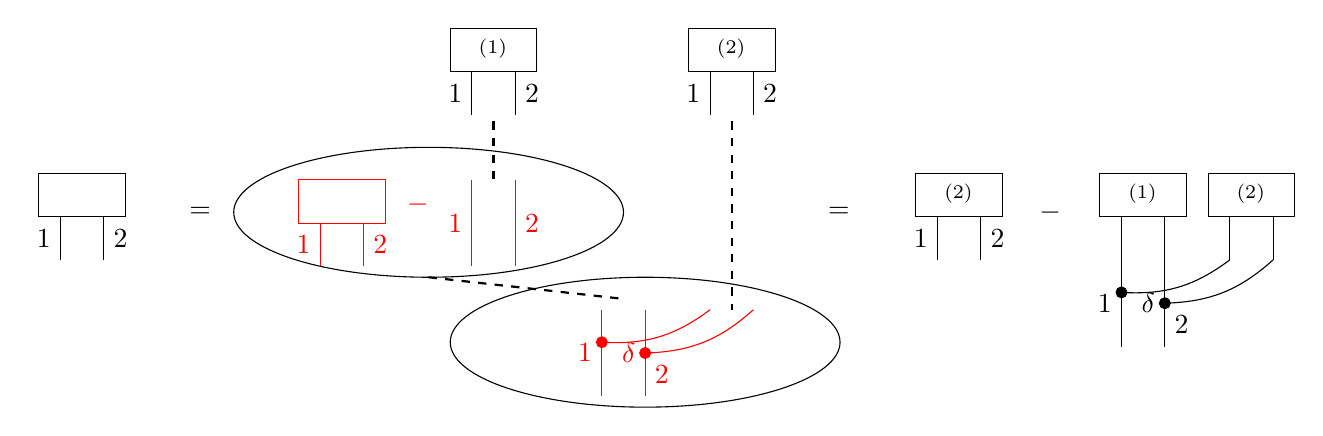
\begin{tikzpicture}[scale=0.275] % , baseline = -3.5pt



\begin{scope}[shift={(-19,-1.7)}]
		%\draw[] (-1,2.2) ellipse (4 and 2.5);
	  	\draw  (-3,2) rectangle (1,4);
		\node at (-1,1.9) [above] {${\exformula}$};
		\draw (-2,2) -- (-2,0) node[midway,left] {$\catvariableof{1}$};
		\draw (0,2) -- (0,0) node[midway,right] {$\catvariableof{2}$};	
		\node at (3.5,2.2)[right]  {$=$};
\end{scope}

\draw[] (-4,0.5) ellipse (9 and 3);
   	\begin{scope}[shift={(-2,-2)}]
  		\draw[\skeletoncolor] (-8,2) rectangle (-4,4);
		\node at (-6,2) [above,\skeletoncolor] {$\ones$};
		\draw[\skeletoncolor] (-7,2) -- (-7,0) node[midway,left] {$\catvariableof{1}$};
		\draw[\skeletoncolor] (-5,2) -- (-5,0) node[midway,right] {$\catvariableof{2}$};
	\end{scope}
	
	\draw[\skeletoncolor] (-2,2) -- (-2,-2) node[midway,left] {$\catvariableof{1}$};
	\draw[\skeletoncolor](0,2) -- (0,-2) node[midway,right] {$\catvariableof{2}$};
	\node[\skeletoncolor] at (-4.5,0) [above] {$-$};
\draw[thick,dashed] (-4,-2.5) -- (5,-3.5);
%\draw[] (6,-2.5) -- (1,-2.5);

%% Into negation core
\draw[thick,dashed] (-1,4.7) -- (-1,2);%-4,3.5);

%% Into conjunction core
\draw[thick,dashed] (10,4.7) -- (10,-4);%(6,-2.5);


\begin{scope}[shift={(10,-6)}]
	\draw[] (-4,0.5) ellipse (9 and 3);
	\begin{scope}[shift={(-4,0)}]
		\renewcommand{\skeletoncolor}{red}
	\node at (0,0) [left,\skeletoncolor] {$\delta$};
	\draw[\skeletoncolor]  (0,2) -- (0,0);% node[midway,left] {$\placeholderof{1}$};
	\draw[fill,\skeletoncolor] (0,0) circle (0.25cm);
	\draw[\skeletoncolor] (0,0) -- (0,-2) node[midway,right] {$\catvariableof{2}$};
	\draw[\skeletoncolor] (5,2) to[bend left=20] (0,0);


	\draw[fill,\skeletoncolor] (-2,0.5) circle (0.25cm);
	\draw[\skeletoncolor] (3,2) to[bend left=20] (-2,0.5);
	\draw[\skeletoncolor] (-2,2) -- (-2,-2) node[midway,left] {$\catvariableof{1}$};
	\end{scope}
\end{scope}



\begin{scope}[shift={(0,5)}]
		%\draw[] (-1,2.2) ellipse (4 and 2.5);
	  	\draw  (-3,2) rectangle (1,4);
		\node at (-1,1.9) [above] {${\secexformula^{(1)}}$};
		\draw (-2,2) -- (-2,0) node[midway,left] {$\catvariableof{1}$};
		\draw (0,2) -- (0,0) node[midway,right] {$\catvariableof{2}$};	
\end{scope}

\begin{scope}[shift={(11,5)}]
		%\draw[] (-1,2.2) ellipse (4 and 2.5);
	  	\draw  (-3,2) rectangle (1,4);
		\node at (-1,1.9) [above] {${\secexformula^{(2)}}$};
		\draw (-2,2) -- (-2,0) node[midway,left] {$\catvariableof{1}$};
		\draw (0,2) -- (0,0) node[midway,right] {$\catvariableof{2}$};	
		
\end{scope}




\node at (14,0.5)[right]  {$=$};


\begin{scope}[shift={(29,0)}]

\begin{scope}[shift={(-7.5,-1.7)}]
		%\draw[] (-1,2.2) ellipse (4 and 2.5);
	  	\draw[]  (-3,2) rectangle (1,4);
		\node at (-1,1.9) [above] {${\secexformula^{(2)}}$};
		\draw[] (-2,2) -- (-2,0) node[midway,left] {$\catvariableof{1}$};
		\draw[] (0,2) -- (0,0) node[midway,right] {$\catvariableof{2}$};	
		\node at (2.25,2.2)[right]  {$-$};		
\end{scope}


\begin{scope}[shift={(1,-3.7)}]
%	\renewcommand{\skeletoncolor}{\conjunctioncolor}
	\node at (0,0) [left] {$\delta$};
	\draw[]  (0,2) -- (0,0);% node[midway,left] {$\placeholderof{1}$};
	\draw[fill] (0,0) circle (0.25cm);
	\draw[] (0,0) -- (0,-2) node[midway,right] {$\catvariableof{2}$};
	\draw[] (5,2) to[bend left=20] (0,0);


	\draw[fill] (-2,0.5) circle (0.25cm);
	\draw[] (3,2) to[bend left=20] (-2,0.5);
	\draw[] (-2,2) -- (-2,-2) node[midway,left] {$\catvariableof{1}$};
\end{scope}


\begin{scope}[shift={(1,-1.7)}]
		%\draw[] (-1,2.2) ellipse (4 and 2.5);
	  	\draw  (-3,2) rectangle (1,4);
		\node at (-1,1.9) [above] {${\secexformula^{(1)}}$};
		\draw[] (-2,2) -- (-2,0); % node[midway,left] {$\catvariableof{1}$};
		\draw[] (0,2) -- (0,0); % node[midway,right] {$\catvariableof{2}$};	
	
\end{scope}
	
\begin{scope}[shift={(6,-1.7)}]
		%\draw[] (-1,2.2) ellipse (4 and 2.5);
	  	\draw[]  (-3,2) rectangle (1,4);
		\node at (-1,1.9) [above] {${\secexformula^{(2)}}$};
		\draw[]  (-2,2) -- (-2,0); % node[midway,left] {$\catvariableof{1}$};
		\draw[]  (0,2) -- (0,0); % node[midway,right] {$\catvariableof{2}$};	
	
\end{scope}

\end{scope}



	
	
\end{tikzpicture}
\end{center}
\caption{
	Example of a decomposition by effective calculus of a formula $\exformula(\catvariableof{1},\catvariableof{2}) = \textcolor{blue}{\lnot} \secexformula^{(1)}(\catvariableof{1},\catvariableof{2}) \textcolor{red}{\land}  \secexformula^{(2)}(\catvariableof{1},\catvariableof{2})$ into a sum of contractions.}
	\label{fig:DecompositionExample}
\end{figure}




\subsection{Applications in Machine Learning}

The neural paradigm of Machine Learning describes the relevance of sparse function to be effective models in the sense of learning and approximation.

% Neural Paradigm by Tensor Network Decompositions
Our model of the neural paradigm are tensor network decompositions, seen as decomposition of functions into smaller functions, which take each other as input.
Summations along input axis are avoided, when having directed and binary tensor networks with basis calculus interpretation.

% Basis Calculus
We have already observed in Theorem~\ref{the:basisCalculus}, that the value of discrete maps can be calculated by contractions of the directed binary relation encodings.
This has been framed as Basis Calculus.
What is more, tensor network decompositions into directed binary tensors correspond with representation of functions as compositions of smaller functions.
We can understand each composition as marking a neuron in an architecture and thus have established a neural perspective on binary directed tensor networks.
